%%%%%%%%%%%%%%%%%%%%%%%%%%%%%%%%%%%%%%%%%%%%%%%%%%%%%%%%%%%%%%%%%%%%
%Imperial College
\documentclass[a4paper,11pt,twoside]{article}
\usepackage[left=2.5cm,right=2cm,top=2cm,bottom=2cm]{geometry}

%%%%%%%%%%%%%%%%%%%%%%%%%%%%%%%%%%%%%%%%%%%%%%%%%%%%%%%%%%%%%%%%%%%%%
% Paragraph
\usepackage[parfill]{parskip}

% Images
\usepackage{graphicx} 
\usepackage{caption}
\usepackage{subcaption}

% URLs
\usepackage{hyperref}

% Maths
\usepackage{amsmath}
\usepackage{xfrac}

% Code listings
\usepackage{listings}
% Code styling
\usepackage{MnSymbol}
\lstset{prebreak=\raisebox{0ex}[0ex][0ex]{\ensuremath{\rhookswarrow}}}
\lstset{postbreak=\raisebox{0ex}[0ex][0ex]{\ensuremath{\rcurvearrowse\space}}}
\lstset{breaklines=true, breakatwhitespace=true}
\lstset{numbers=left, numberstyle=\scriptsize}
\lstset{language=Python, basicstyle=\ttfamily}

% Clever referencing
\usepackage{cleveref}

%%%%%%%%%%%%%%%%%%%%%%%%%%%%%%%%%%%%%%%%%%%%%%%%%%%%%%%%%%%%%%%%%%%%%
\begin{document} 
\title{MCMC in Action}

\date{\today} 
\author{Dakshina Scott} 
\maketitle

%%%%%%%%%%%%%%%%%%%%%%%%%%%%%%%%%%%%%%%%%%%%%%%%%%%%%%%%%%%%%%%%%%%%%
\begin{abstract} 
Rejection sampling and the Metropolis-Hastings algorithm were both
implemented in the Python programming language and applied to the univariate
Gaussian probability distribution for a parameter in a toy problem. Comparing
these results the benefits of the latter algorithm were seen, and thus it was
used to generate samples from the bivariate distribution for another toy
problem with two unknown parameters.
The samples were used, via maximum likelihood estimates, to find
Monte Carlo estimates for the parameters of the distribution, which were then
compared to those found analytically. The results were found to match well, with an
analytical solution of 
$\theta = \begin{bmatrix} 
		-0.012 \\ 
	1.329 \end{bmatrix}$ and a Monte Carlo estimate $\theta_{MC} = \begin{bmatrix} 
		-0.012 \\ 
	1.329 \end{bmatrix}$, suggesting that the algorithm performed well.  

\end{abstract}

%%%%%%%%%%%%%%%%%%%%%%%%%%%%%%%%%%%%%%%%%%%%%%%%%%%%%%%%%%%%%%%%%%%%
\tableofcontents

%%%%%%%%%%%%%%%%%%%%%%%%%%%%%%%%%%%%%%%%%%%%%%%%%%%%%%%%%%%%%%%%%%%%%
\section{Background} 
Markov Chain Monte Carlo (MCMC) can be used to solve problems which would
otherwise not be solvable - such as intractable integrations or sampling from
complicated multivariate probability distributions.  

While the idea of Monte Carlo simulations has been
around for much longer, MCMC has flourished since the rise of computers allowed
much larger simulations. It was originally developed by Metropolis et al. at Los Alamos in
1953 to investigate the equation of state for substances consisting of
individual interacting molecules \cite{metropolis}. Today Markov Chain Monte
Carlo methods are used for many applications in physics and particularly statistical
mechanics, for example in simulating the Ising model\cite{statphys}.

\subsection{Monte Carlo Methods}
Monte Carlo methods use random numbers to solve problems.  A Monte Carlo method
may be more specifically defined as
"representing the solution of a problem as a parameter of a hypothetical
population, and using a random sequence of numbers to construct a sample of the
population, from which statistical estimates of the parameter can be found"
\cite{halton}.  

A very simple example is a Monte Carlo estimate for the value of $\pi$. Assume we have a
circle of radius one, contained exactly within a square ranging [-1, 1]. The
probability of random points from a uniform distribution within this range
landing in the circle is given by:
\begin{equation}
	P(inside) = \theta = \frac{\text{area of circle}}{\text{area of square}} =
	\frac{\pi}{4}.
\end{equation}
As there are only two possible outcomes for each simulation - a point lands
either inside or outside of the circle - a  population of N points can be
described by a binomial distribution in which a 'success' is a point landing within
the circle:
\begin{equation}
	I \sim \mathcal{B}(N, \theta)
\end{equation}
where $I$ is the number of successes.
Thus we have represented the solution of our problem as a parameter of a
hypothetical population, that is a binomial population with unknown probability
of success.
We can estimate $\theta$ using its maximum-likelihood estimate \cite{som}, based
on the number of success we observed in our random sampling:
\begin{equation}
	\theta = \frac{I}{N},
\end{equation}

so a Monte Carlo estimate for $\pi$ is given by
\begin{equation}
	\pi_{MC} = 4 \theta = 4 \frac{I}{N}.
\end{equation}

\subsection{Rejection Sampling}
Rejection sampling is a particular type of Monte Carlo method which can be used
if the target distribution can be evaluated, at least to within a normalization
constant. 

A random number $r$ is generated from some proposal distribution, $Q(\theta)$. A
corresponding random number is generated from a uniform distribution in the
range [0,$Q(\theta = r)$], representing a value on the y-axis. Both the
proposal distribution and the target distribution, $P(\theta|x)$, are
evaluated at this value. The probability of 'accepting' the sample is given by
$\frac{P(\theta = r|x)}{Q(\theta = r)}$ - in practice this is implemented by accepting the
sample if $y < P(\theta = r|x)$, and rejecting otherwise. The accepted points are
effectively a series of samples from the target distribution. From these
samples using the maximum-likelihood estimates for mean and variance gives the
Monte Carlo estimates for said quantities. It is important that $Q(\theta) >
P(\theta|x)$ for every theta value. For simplicity, a uniform distribution is often used.

\subsection{Markov Chains \& The Metropolis-Hastings Algorithm}
Markov chains describe the probability of transitions between different states
in a system. Specifically, for a sequence to be a Markov chain, the
probability of transitioning to a state must depend only on the current state
and not on any previous states.

In Markov Chain Monte Carlo a Monte Carlo method is used where the sequence of
states is a Markov Chain. There are a number of algorithms which achieve this
(see, for example, Gibbs sampling).
Here we have used the Metropolis-Hastings algorithm, in which the next state is
given by a proposal distribution, similar to that described above. However,
in this case the proposal distribution is always centred on the current state.
This results in a sequence of samples constituting a Markov Chain with the
target distribution as its equillibrium distribution.

\section{Univariate Target Distribution}
Here we use a toy problem based on set of measurements of size $N = 10$ (shown
in \cref{sec:data}) with sample mean $\bar{x} = 0.464$ and variance $\sigma^2 =
0.1$.
These data are randomly generated from a Gaussian distribution, and are used in
place of actual experimental results to update our knowledge about a
distribution from the prior to the posterior. We use a Gaussian prior with mean
$\mu_{prior} = 0$ and variance $\Sigma^{2} = 1.0$.

\subsection{Analytical Solution}
In this case we have a simple Gaussian prior and likelihood, for which it can be shown
that the resulting posterior is also a Gaussian (see \cref{sec:posterior}).
Because we know the form of the equation for a gaussian distribution, it can be
seen that the posterior mean and standard deviation are given by:
\begin{equation}
	\mu_{post} = \frac{\Sigma^2}{\sfrac{\sigma^2}{N} + \Sigma^2} \bar{x} = 0.463,
\end{equation}

\begin{equation}
	\sigma_{post} = \left( \frac{1}{\Sigma^2} + \frac{N}{\sigma^2} \right)^{-\frac{1}{2}} = 0.032.
\end{equation}

This analytical solution gives us something to which our MCMC results can be
compared. However, in real world applications of MCMC this of course would not
be available.

\subsection{Rejection Sampling} 
First a simple Monte Carlo method - rejection sampling - was applied to our toy
problem.
\begin{figure}[ht]
	\centering
	\begin{subfigure}[t]{0.4\textwidth}
		\centering
		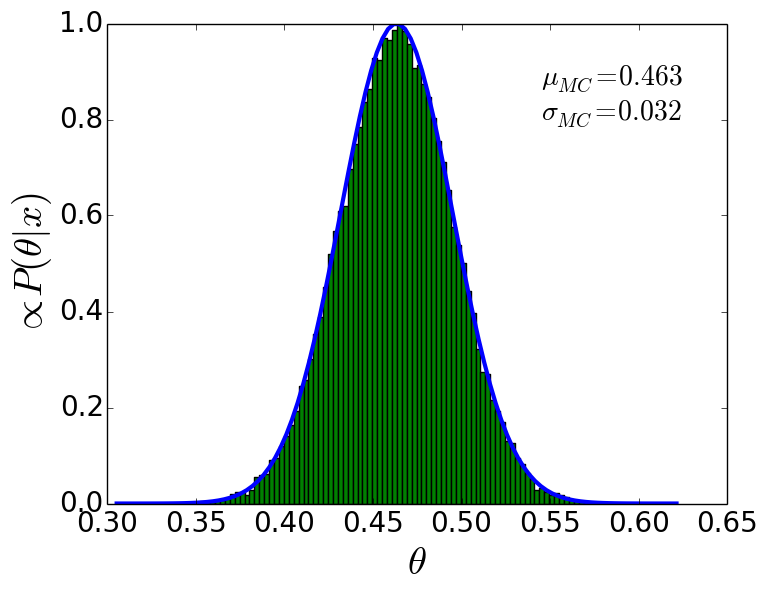
\includegraphics[width=\textwidth]{rejection.png}
		\caption{The histogram in green represents the distribution
			found by rejection sampling. The Monte Carlo mean and standard
			deviation are found to be $\mu_{MC} = 0.463$ and $\mu_{MC} = 0.032$.
			The blue line is the analytical distribution.}
		\label{fig:rejection}
	\end{subfigure}
	~
	\begin{subfigure}[t]{0.4\textwidth}
		\centering
		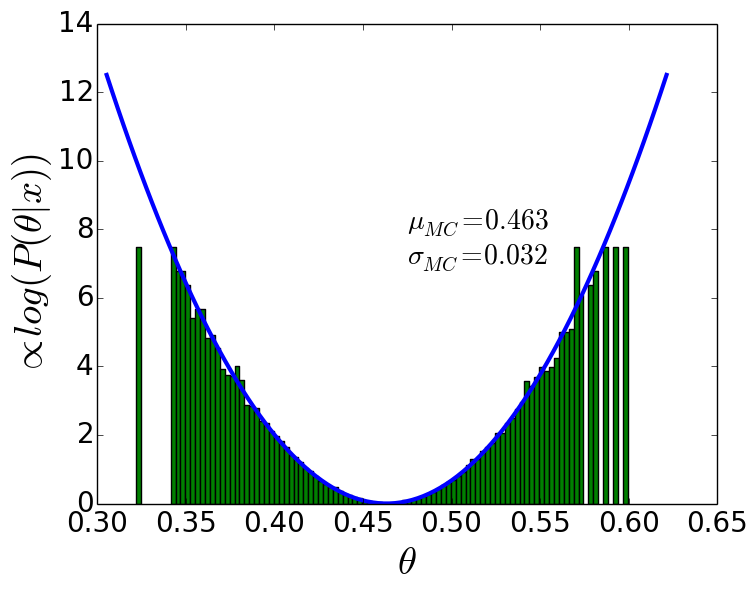
\includegraphics[width=\textwidth]{rejlog.png}
		\caption{A log-plot makes it easier to see the discrepencies at
			the extremities of the plot. These are due to the finite
		domain over which samples are taken using this method.}
		\label{fig:rejlog}
	\end{subfigure}
	\caption{}\label{fig:rejplots}
\end{figure}

In figure \ref{fig:rejection}, the results appear to fit the analytical curve well.
However, plotting the logarithm of the results allows us to see clearly differences at
the edges of our Monte Carlo sample - this is because we can't take samples over
an infinite domain, and in this algorithm we must choose definite cut-off
points. The wider the domain the smaller the effect of this will be, but the
number of rejected candidate points will be larger. As there always has to be a
cut-off somewhere, this is an area where the Metropolis-Hastings algorithm will
be more effective. 

\subsection{Metropolis-Hastings Algorithm} 
The Metropolis-Hastings algorithm was then applied to the same problem, using a
Gaussian proposal distribution. 
\begin{figure}[ht]
	\centering
	\begin{subfigure}[t]{0.4\textwidth}
		\centering
		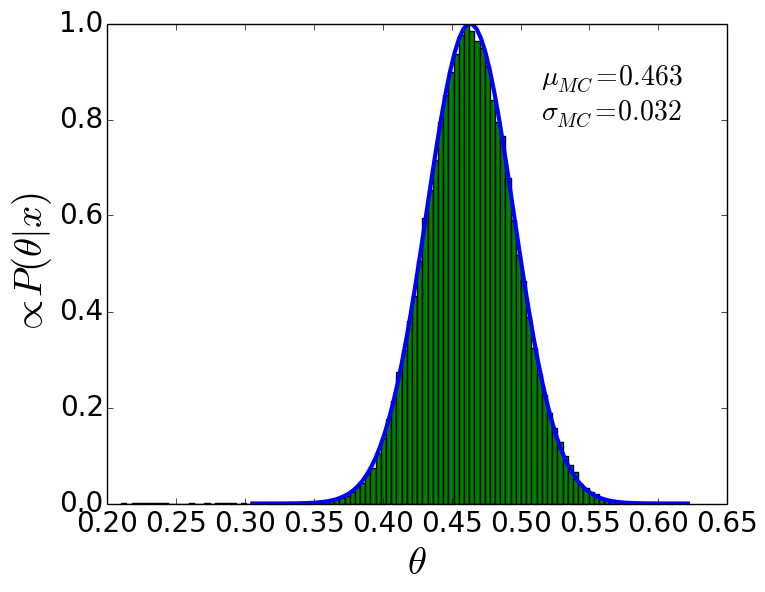
\includegraphics[width=\textwidth]{metropolishastings.png}
		\caption{The histogram in green represents the distribution
			found by the Metropolis-Hastings algorithm. The Monte Carlo mean and standard
			deviation are found to be $\mu_{MC} = 0.463$ and $\sigma_{MC} = 0.032$.
			The blue line is the analytical distribution.}
		\label{fig:metropolis}
	\end{subfigure}
	~
	\begin{subfigure}[t]{0.4\textwidth}
		\centering
		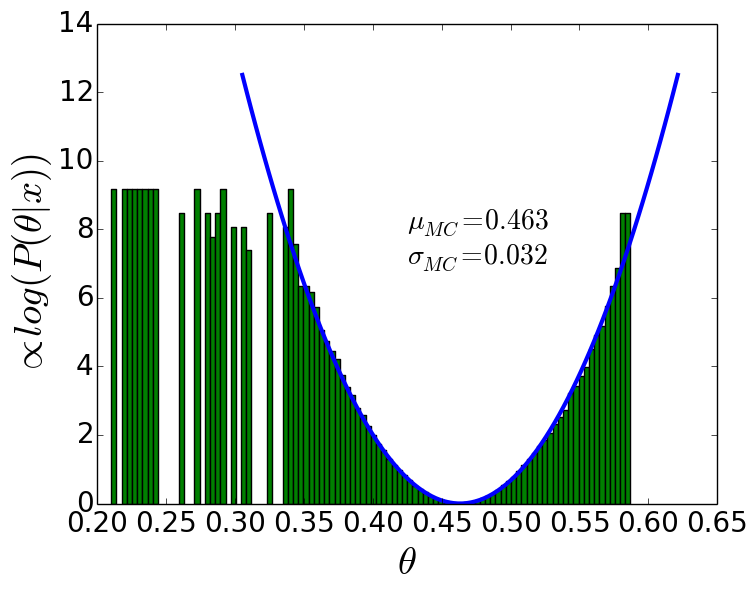
\includegraphics[width=\textwidth]{mhlog.png}
		\caption{A log-plot of the Metropolis-Hastings results shows
		that the sample is more consistent with the analytical solution,
	as compared with figure \ref{fig:rejlog}.}
		\label{fig:mhlog}
	\end{subfigure}
	\caption{}\label{fig:mh}
\end{figure}

It can be seen from figure \ref{fig:mhlog} that there are some samples which are clear
outliers from the distribution. This is due to a poor starting value for the
chain. Starting far from the high-probability parts of the distribution results
in a disproportionate number of extreme values being accepted in the early
iterations. These early samples are sometimes discarded as burn-in. There is
some debate over how best to determine the length of the burn-in period, and
indeed whether a burn-in should be used at all \cite{handbook}.
A simple qualitative approach for determining the length of the burn-in 
would be to run multiple chains from very different starting
positions. When these chains meet, one would expect the chains to have
converged to the target distribution and so all previous points can be
discarded. 

While this approach provides some evidence that the chains are converging
regardless of starting position, it should not be regarded as definitive as not
all starting positions can be tested. For some multi-peak distributions it is
conceivable that multiple chains with very different initial states may become
stuck in the same area for some time.

\begin{figure}[!ht]
	\centering
	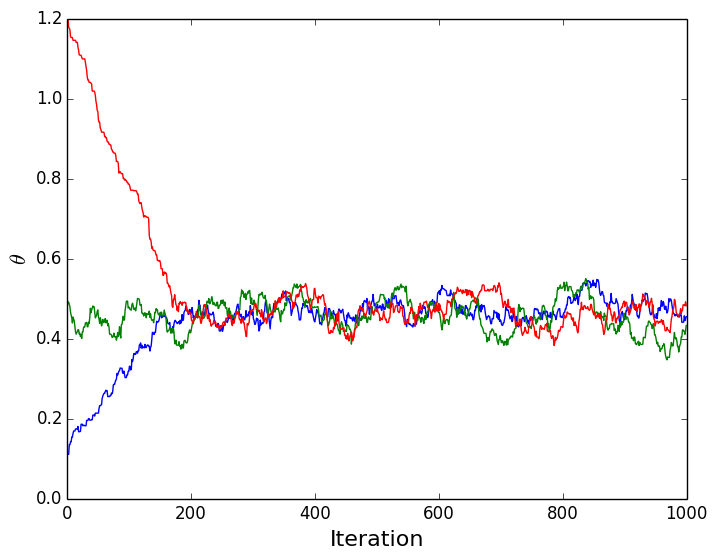
\includegraphics[width=0.8\textwidth]{convergence.png}
	\caption{Starting the chain from three very different states gives us
	an idea of how the chain converges. We see the chains meet after
	about 200 iterations, suggesting that the chain converges around here.}
	\label{fig:convergence}
\end{figure}
In figure \ref{fig:convergence} we see three very different starting $\theta$
values which appear to converge after about 200 iterations, so we take 200
iterations as the burn-in period, as is seen in figure \ref{fig:mhplotsb}.
\begin{figure}[!ht]
	\centering
	\begin{subfigure}[t]{0.4\textwidth}
		\centering
		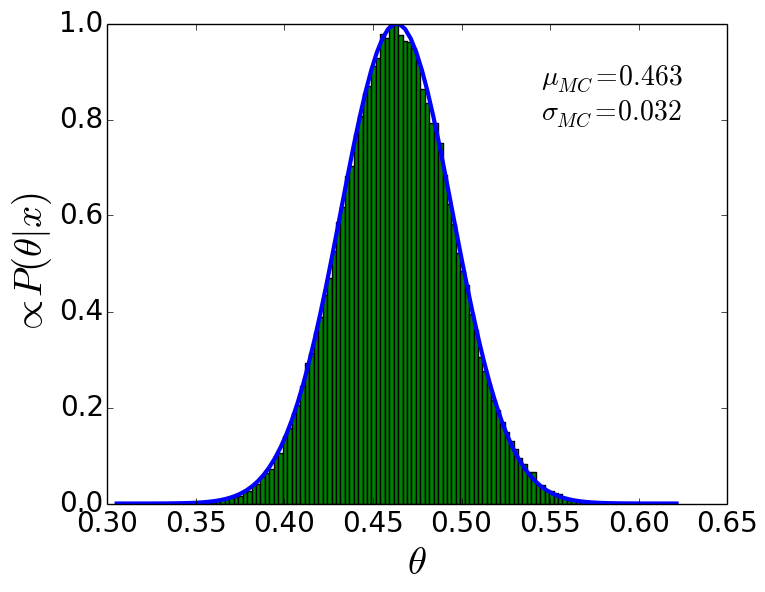
\includegraphics[width=\textwidth]{metropolishastings-burnin.png}
		\caption{The results from the Metropolis-Hastings algorithm
		with the first 200 iterations removed as burn-in. }
		\label{fig:metropolisb}
	\end{subfigure}
	~
	\begin{subfigure}[t]{0.4\textwidth}
		\centering
		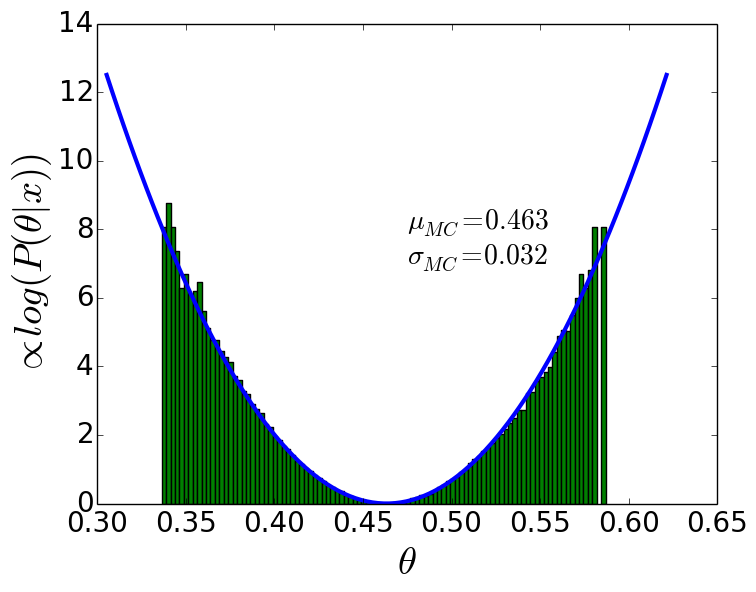
\includegraphics[width=\textwidth]{mhlog-burnin.png}
		\caption{A log plot of the Metropolis-Hastings results with
		burn-in removed. Although the plot appears different, $\mu$
		remains the same to 3 significant figures, and the standard deviation
		is also unaffected at this precision.}
		\label{fig:mhlogb}
	\end{subfigure}
	\caption{}\label{fig:mhplotsb}
\end{figure}
In figure \ref{fig:mhlogb} it appears that although closer than the rejection
sampling case, there are still some issues at extreme $\theta$ values. It can be seen that
the histogram slightly overshoots the analytical plot at the edges - as this is a log
plot this suggests that the more extreme values are under-represented in our
sample.

\section{Bivariate Target Distribution} 
Consider the linear model
\begin{equation}
	y = F\theta + \epsilon
\end{equation}
where y is a vector containing our data, $\theta$ is a vector of unkown
parameters, F is the design matrix and $\epsilon$ is a vector containing the
noise. Let's assume that the noise is randomly gaussian distributed with zero
mean and zero correlation, then the likelihood function can be shown to take the form
\begin{equation}
	p(y|\theta) = \mathcal{L}_0 \exp\left[-\frac{1}{2}(\theta - \theta_0)^tL(\theta - \theta_0)\right],
\end{equation}
where $L$ is the likelihood fisher matrix, $\mathcal{L}_1$ is a constant, and
$\theta_0$ is dependent on $L$ and constants related to the linear model above
(see \cref{sec:2dlikelihood}).

Also say we have a Gaussian prior with zero mean and Fisher matrix $P$, i.e.
\begin{equation}
	p(\theta) = \frac{|P|^{\sfrac{1}{2}}}{(2\pi)^{\sfrac{n}{2}}} \exp \left[ \frac{1}{2} \theta^t P \theta \right].
\end{equation}

\subsection{Analytical Solution}
Using Bayes theorem the posterior can be shown to follow
\begin{equation}
	p(\theta|y) \propto \exp \left[ -\frac{1}{2} (\theta - \bar{\theta})^t \mathcal{F} (\theta - \bar{\theta}) \right],
\end{equation}
where $\mathcal{F} = L + P$ and $\bar{\theta} = \mathcal{F}^{-1}L\theta_0$ (see \cref{sec:2dposterior}).
From this it is clear that $\bar{\theta}$ is the posterior mean and
$\mathcal{F}$ is the posterior Fisher matrix, but only because both the prior
and the likelihood had the same (Gaussian) form - resulting in a Gaussian
posterior.

While these results apply to the multivariate case in general, here we
specialize to the bivariate case. Specifically we take a prior with Fisher matrix
	$ P = \begin{bmatrix}
		10^{-2} & 0 \\
		0 & 10^{-2}
	\end{bmatrix}, $
and a set of simulated data points with noise (see \cref{sec:data}).
From this we find that the posterior mean, 
	$\bar{\theta} = \begin{bmatrix} 
		\theta_1 \\ 
		\theta_2 \end{bmatrix} = \begin{bmatrix} 
		-0.012 \\ 
	1.329 \end{bmatrix}$.

\begin{figure}[!ht]
	\centering
	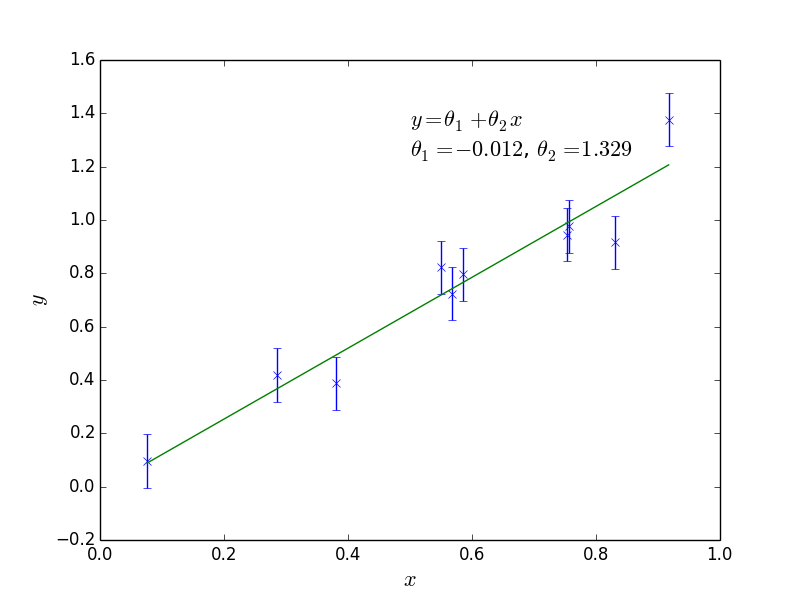
\includegraphics[width=0.8\textwidth]{2ddata.png}
	\caption{In blue are the simulated data with their associated
	error bars. The green line is the linear model $y = \theta_1 + \theta_2
	x$ with the parameters $\theta_1$ and $\theta_2$ found analytically.}
	\label{fig:model}
\end{figure}

\subsection{Metropolis-Hastings Algorithm} 

The Metropolis-Hastings algorithm was then applied to this bivariate posterior
distribution. The program includes a preliminary run - this is done in order
to find a rough outline of the posterior distribution. From this the
orientation of the elliptical distribution can be approximated, which is used in order
to transform the distribution to a unit circle. Samples are taken from this
using Metropolis-Hastings, and then transformed back to the original
distribution, as seen in figure \ref{fig:rot-unrot}. 
This makes the choice of proposal distribution simpler and the
algorithm more efficient - it is easiest to choose the proposal distribution
such that the standard deviations are specified in the x and y directions.
However if the ellipse of our desired distribution is not aligned with the axes
then this will reduce the efficiency of the mixing. Transforming the ellipse
not only aligns it to the axes (and thus to the proposal distribution) but also
means we can use the same proposal standard devation in along each axis.
\begin{figure}[!ht]
	\centering
	\begin{subfigure}[t]{0.4\linewidth}
		\centering
		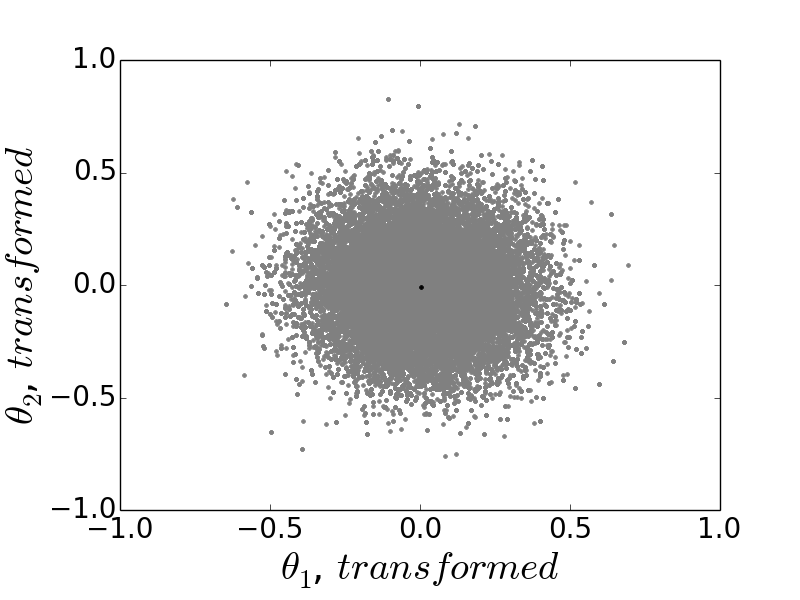
\includegraphics[width=\textwidth]{rot.png}
		\caption{Metropolis-Hastings samples as they appear when
		transformed. The proposal standard deviations can now be parallel to
		the axes and easily explore the whole target distribution.}
		\label{fig:rot}
	\end{subfigure}
	~
	\begin{subfigure}[t]{0.4\linewidth}
		\centering
		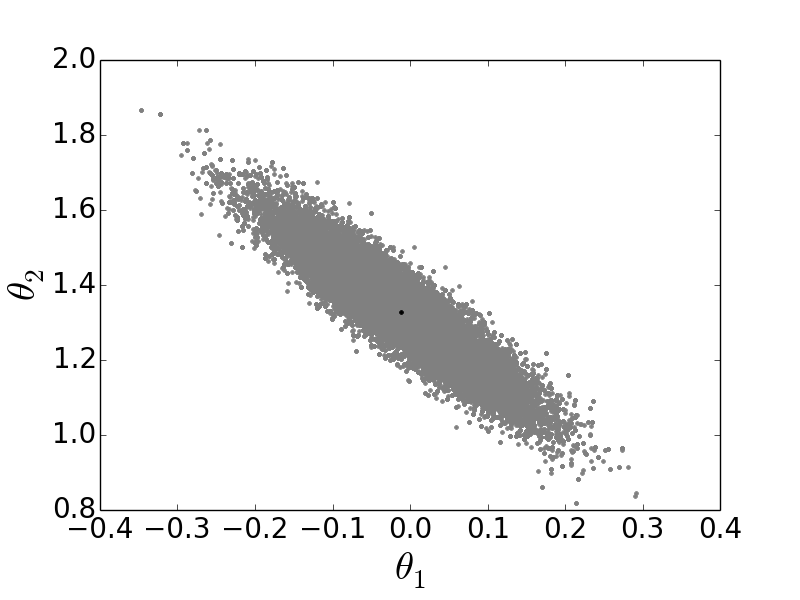
\includegraphics[width=\textwidth]{unrot.png}
		\caption{Metropolis-Hastings samples transformed back to
		an ellipse. Proposal standard deviations are hard to optimise
		for the distribution in this form. }
		\label{fig:unrot}
	\end{subfigure}
	\caption{}\label{fig:rot-unrot}
\end{figure}

Another benefit of using a preliminary run is that the resulting mean can be used
as the initial $\theta$ in the main run. This may reduce mixing time, and
remove the need for a burn-in\cite{handbook}.

The standard deviation was chosen such the the acceptance rate $a \approx 0.35$
as according to Gelman et. al this is the optimal value for a
normal target distribution in two dimensions \cite{acceptance}.
The results are shown below in figure \ref{fig:marginalized} with confidence regions indicating those
regions containing 67\%, 95\% and 99\% of the samples.

%\begin{figure}[!ht]
%	\centering
%	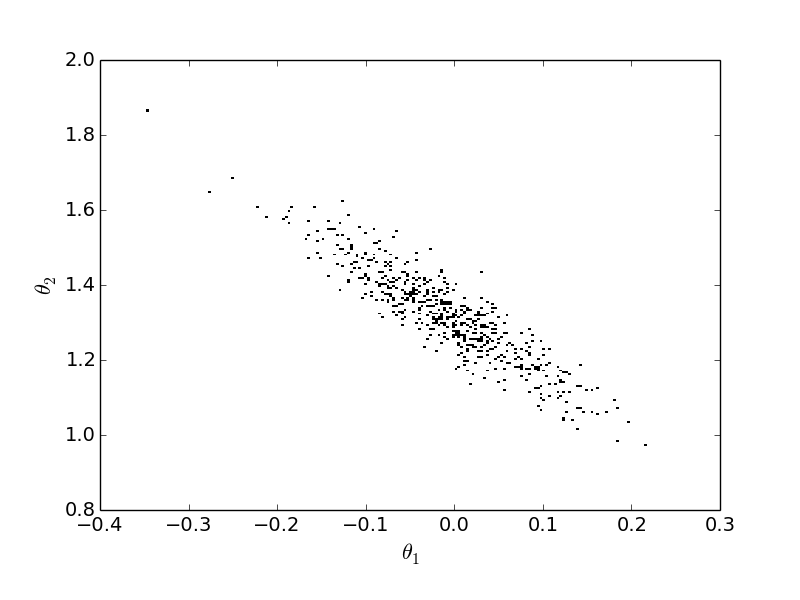
\includegraphics[width=0.8\textwidth]{equalweight.png}
%	\caption{Equal weight samples allow us to visualize the density even in the most dense regions.}
%	\label{fig:equalweight}
%\end{figure}


\begin{figure}[!ht]
	\centering
	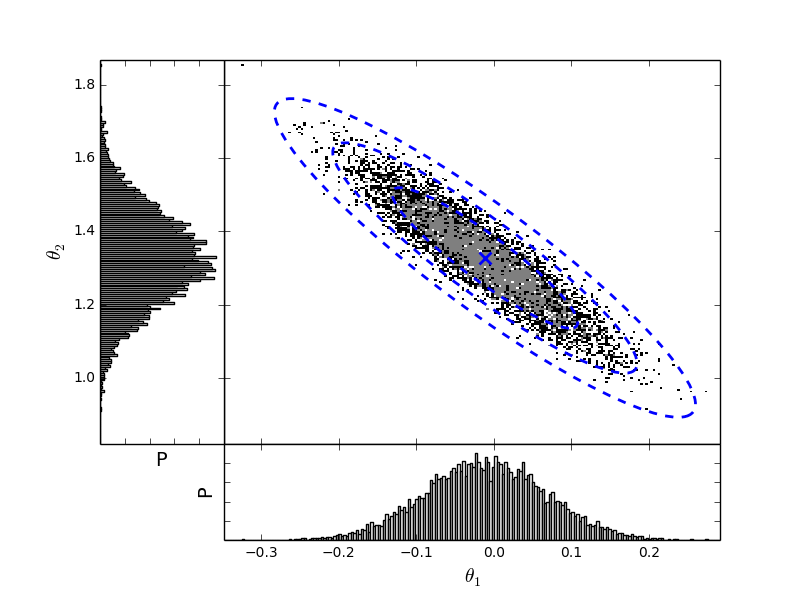
\includegraphics[width=\textwidth]{marginalized.png}
	\caption{On the top right is a plot of Metropolis-Hastings samples, shaded to
	represent $1-$, $2-$ and $3-\sigma$ confidence regions as approximated
	numerically. This is overlaid with the analytically calculated confidence
	regions outlined in blue. Alongside are the one-dimensional marginalized posterior
	distributions for each parameter.}
	\label{fig:marginalized}
\end{figure}
The Monte Carlo estimate for the parameter was found to be $\theta_{MC} = \begin{bmatrix} 
		-0.012 \\
	1.329 \end{bmatrix}$, which matches the analytical result to 3 decimal places.

Both the numerically approximated and
analytically calculated confidence regions, as well as marginalized
distributions for each parameter are shown in figure \ref{fig:marginalized}. The numerical approximation was made under
the assumption that the population always decreases radially out from the mean.
As we have a finite sample size this in practice is not always the case, and so
the confidence regions are not as clear as they would be if we had not used
such an assumption. However they serve to visually give us a clearer idea of of
how well our MCMC samples fit the target distribution. Checking the numerical
approximation, the $1-$, $2-$ and $3-\sigma$ regions contain 67.9\%, 94.4\% and
97.2\% of the samples respectively - indicating that the aforementioned
assumption about our distribution of samples is imperfect, but very close in the more populated areas.

\begin{figure}[!ht]
	\centering
	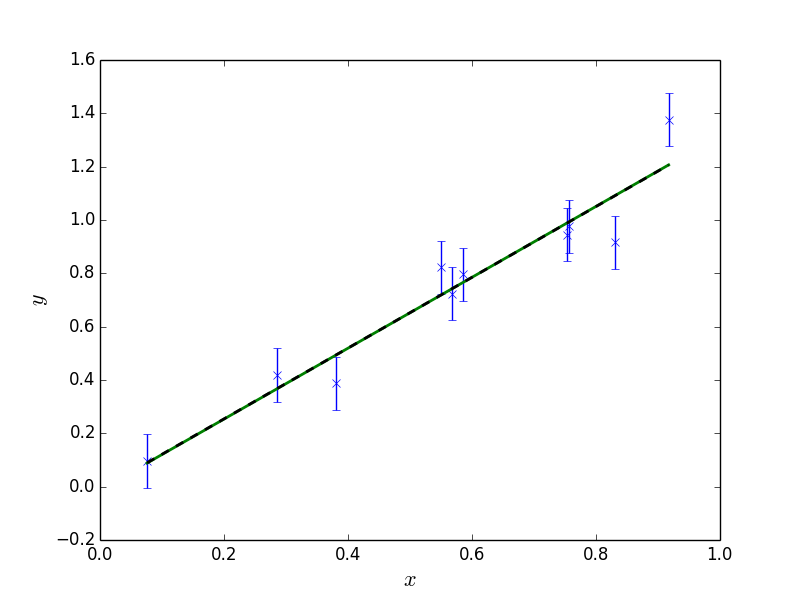
\includegraphics[width=0.8\textwidth]{2ddata-mcmc.png}
	\caption{As above, the green line is the analytical solution. The
	dashed black line shows the model found using the Metropolis-Hastings
	method.}
	\label{fig:model-mcmc}
\end{figure}

\section{Conclusion}
We have seen that the Metropolis-Hastings algorithm produces better results in
the one-dimensional case than rejection sampling. On applying this to a
two-dimensional toy problem it was to produce results which match the
analytical solution well, suggesting that it would be a good choice of MCMC
method for future problems. The analytical solution to our problem was found to be $\theta = \begin{bmatrix} 
		-0.012 \\ 
	1.329 \end{bmatrix}$ and the Monte Carlo estimate $\theta_{MC} = \begin{bmatrix} 
		-0.012 \\ 
	1.329 \end{bmatrix}$. However, a preliminary run was used to improve the
results of the main run, which takes extra time and may not always be
convenient. In order to achieve accuracy to 3 decimal places 300,000 iterations
of Metropolis-Hastings were used. Running this takes some time, and it would be
worthwhile to focus some more on improving the efficiency of the program (for
example implementing it in C instead of Python may improve it's speed).

%%%%%%%%%%%%%%%%%%%%%%%%%%%%%%%%%%%%%%%%%%%%%%%%%%%%%%%%%%%%%%%%%%%%%
\appendix 
\label{appendix}

\section{One-Dimensional Likelihood Function}
\label{sec:likelihood}
The likelihood distribution for a set of $N$ measurements is given by the product of the likelihood for each measurement:
\begin{align*}
	\mathcal{L}(\theta) &= \prod_{i=1}^{N} \frac{1}{\sqrt{2\pi}\sigma}\exp\left(-\frac{1}{2}\frac{(\theta - \hat{x}_i)^2}{\sigma^2}\right)
	\\ &= \left(\frac{1}{\sqrt{2\pi}\sigma}\right)^N \exp\left(-\frac{1}{2}\sum_{i=1}^{N}(\frac{\theta - \hat{x}_i)^2}{\sigma^2}\right).
\end{align*}
Taking, for now, just the exponent, and using that $\bar{x} = \frac{1}{N} \sum_i \bar{x}_i \Rightarrow \sum_i \hat{x}_i = N \bar{x}$:
\begin{align*}
	-\frac{1}{2\sigma^2}\sum_i^N(\theta - \hat{x})^2 &= -\frac{1}{2\sigma^2}(N\theta^2 - 2\theta \sum_i^N\hat{x}_i + \sum_i^N \hat{x}_i^2) 
	\\ &= -\frac{1}{2\sigma^2}(N\theta^2 - 2\theta N \bar{x} + \sum_i^N \hat{x}_i^2) 
	\\ &= -\frac{N}{2\sigma^2} (\theta^2 - 2\theta \bar{x} [ + \bar{x}^2 - \bar{x}^2]  + \frac{1}{N} \sum_i^N \hat{x}_i^2) 
	\\ &= -\frac{N}{2 \sigma^2} (\theta - \bar{x})^2 - \frac{N}{2 \sigma^2}(\frac{1}{N} \sum_{i=1}^{N} \hat{x}_i^2 - \bar{x}^2).
\end{align*}
So
\begin{align*}
	\mathcal{L}(\theta) &= \left( \frac{1}{\sqrt{2\pi}} \right)^N \exp \left(- \frac{N}{2 \sigma^2}(\frac{1}{N} \sum_{i=1}^{N} \hat{x}_i^2 - \bar{x}^2)\right) \exp \left(-\frac{N}{2 \sigma^2} (\theta - \bar{x})^2 \right)
	\\ &= L_0 \exp \left( -\frac{N}{2 \sigma^2} (\theta - \bar{x})^2 \right),
\end{align*}
where $L_0 = \left( \frac{1}{\sqrt{2\pi}} \right)^N \exp \left(- \frac{N}{2 \sigma^2}(\frac{1}{N} \sum_i \hat{x}_i^2 - \bar{x}^2)\right)$.

\section{Computing the Posterior Probability for Theta}
\label{sec:posterior}
Bayes theorem is given by:
\begin{align*}
	p(\theta|x) = \frac{p(x|\theta)p(\theta)}{p(x)}.
\end{align*}
Ignoring the normalization constant (as it is independent of $\theta$):
\begin{align*}
	p(\theta|x) \propto p(x|\theta)p(\theta).
\end{align*}
We have that
\begin{equation*}
	p(x|\theta) = L_0 \exp \left( -\frac{N}{2 \sigma^2} (\theta - \bar{x})^2 \right),
\end{equation*}
and
\begin{equation*}
	p(\theta) =  \frac{1}{\sqrt{2\pi}}\exp\left(-\frac{1}{2}\frac{\theta^2}{\Sigma^2}\right).
\end{equation*}

From these,
\begin{equation*}
	p(\theta|x) \propto \exp \left[ -\frac{1}{2} \left( \frac{(\theta - \bar{x})^2}{\sfrac{\sigma^2}{N}} +\frac{\theta^2}{\Sigma^2} \right) \right].
\end{equation*}

Taking just the exponent,
\begin{align*}
	\frac{(\theta - \bar{x})^2}{\sfrac{\sigma^2}{N}} + \frac{\theta^2}{\Sigma^2} &= \frac{N}{\Sigma^2\sigma^2} \left[\Sigma^2 (\theta - \bar{x})^2 + \frac{\sigma^2}{N} \theta^2 \right]
	\\ &= \left( \frac{1}{\Sigma^2} + \frac{N}{\sigma^2} \right) \left( \frac{1}{\sfrac{\sigma^2}{N} + \Sigma^2} \right) \left[ (\Sigma^2 + \frac{\sigma^2}{N})\theta^2 - 2\bar{x}\Sigma^2\theta + \Sigma^2\bar{x}^2 \right]
	\\ &= \left( \frac{1}{\Sigma^2} + \frac{N}{\sigma^2} \right) \left( \theta^2 - 2 \frac{\Sigma^2}{\sfrac{\sigma^2}{N} + \Sigma^2} \theta + \frac{\Sigma^2}{\sfrac{\sigma^2}{N} + \Sigma^2} \bar{x}^2 \right).
\end{align*}
The final term above is independent of $\theta$. Thus, as we are dealing with an exponent, we can subtract this term and add its square without losing proportionality. This allows us to complete the square so we have:
\begin{equation*}
	\left( \frac{1}{\Sigma^2} + \frac{N}{\sigma^2} \right) \left( \theta - \frac{\Sigma^2}{\sfrac{\sigma^2}{N} + \Sigma^2} \bar{x} \right)^2.
\end{equation*}

Putting this back inside the exponential we are left with:
\begin{equation*}
	p(\theta|x) \propto \exp \left[ -\frac{1}{2} \left( \frac{1}{\Sigma^2} + \frac{N}{\sigma^2} \right) \left( \theta - \frac{\Sigma^2}{\sfrac{\sigma^2}{N} + \Sigma^2} \bar{x} \right)^2 \right],
\end{equation*}

i.e. the posterior follows a Gaussian distribution with mean $\frac{\Sigma^2}{\sfrac{\sigma^2}{N} + \Sigma^2} \bar{x}$ and standard deviation $\left( \frac{1}{\Sigma^2} + \frac{N}{\sigma^2} \right)^{-\frac{1}{2}}$.

\section{Asymptotic Independence of Posterior on Prior}
For the posterior
\begin{equation*}
	p(\theta|x) \propto \exp \left[-\frac{1}{2} \frac{ \left( \theta - \frac{\Sigma^2}{\sfrac{\sigma^2}{N} + \Sigma^2} \bar{x} \right)^2}{ \left( \frac{1}{\Sigma^2} + \frac{N}{\sigma^2} \right)^{-1}} \right],
\end{equation*}
$
\begin{array}{l l l l}
	\text{as }N \rightarrow \infty, &\quad 
	\\ &\quad \left( \frac{1}{\Sigma^2} + \frac{N}{\sigma^2} \right)^{-1} &\rightarrow \frac{\sigma^2}{N} \quad &\left(\frac{N}{\sigma^2} \gg \frac{1}{\Sigma^2}\right), 
	\\ &\quad \frac{\Sigma^2}{\sfrac{\sigma^2}{N} + \Sigma^2} \bar{x} &\rightarrow \bar{x} \quad &\left(\frac{\sigma^2}{N} \rightarrow 0\right),
\end{array}
$
and the posterior becomes
\begin{equation*}
	p(\theta|x) \propto \exp \left[-\frac{1}{2} \frac{(\theta - \bar{x})^2}{\sfrac{\sigma^2}{N}} \right], 
\end{equation*}
i.e. the likelihood.

\section{Asymptotic Convergence of the Posterior Mean to the MLE Mean for Theta}
The posterior mean is given by:
\begin{equation*}
	\langle \theta \rangle = \int_{-\infty}^{+\infty} \theta p(\theta|x) \mathrm{d} \, \theta.
\end{equation*}
Inserting our equation for the posterior for $N \rightarrow \infty$, we have
\begin{equation*}
	\langle \theta \rangle = \int_{-\infty}^{+\infty} \theta \exp \left[- \frac{1}{2} \frac{(\theta - \bar{x})^2}{\sfrac{\sigma^2}{N}} \right] \mathrm{d} \, \theta. 
\end{equation*}
Making the substitution $y = \theta - \bar{x}$:
\begin{align*}
	\langle \theta \rangle &= \int_{-\infty}^{+\infty} (y+\bar{x})  \exp \left[- \frac{1}{2} \frac{y^2}{\sfrac{\sigma^2}{N}} \right] \mathrm{d} \, y
	\\ &= \int_{-\infty}^{+\infty} \bar{x} \exp \left(- \frac{1}{2}\frac{N}{\sigma^2} y^2 \right) \mathrm{d} \, y,
\end{align*}
as $ y \exp \left(- \frac{1}{2}\frac{N}{\sigma^2} y^2 \right) $ is an odd function.

Substituting back:
\begin{align*}
	\int_{-\infty}^{+\infty} \bar{x} \exp \left[- \frac{N}{\sigma^2} (\theta - \bar{x})^2 \right] \mathrm{d} \, \theta &= \bar{x} \int_{-\infty}^{+\infty} p(\theta|x) \mathrm{d} \, \theta
	\\ &= \bar{x},
\end{align*}
as the integral of a pdf between infinite limits is equal to one. 

\section{2-D Likelihood in Gaussian Form}
\label{sec:2dlikelihood}

For the linear model
\begin{equation*}
	y = F\theta + \epsilon
\end{equation*}
where $\epsilon$ is uncorrelated, the likelihood function is given by
\begin{equation*}
	p(y|\theta) = \frac{1}{(2\pi)^{\frac{d}{2}}\Pi_j\tau_j} \exp\left[-\frac{1}{2}(b - A\theta)^t(b-A\theta)\right],
\end{equation*}
where $A_{ij} = \sfrac{F_{ij}}{\tau_i}$ and $b_i = \sfrac{y_i}{\tau_i}$.

Taking just the variable part of the exponent,
\begin{align*}
	(b - A\theta)^t(b-A\theta) &= (A\theta - b)^t(A\theta - b)
	\\ &= (\theta - A^{-1}b)^tA^tA(\theta - A^{-1}b)
	\\ &= (b - AA^{-1}(A^t)^{-1}A^tb)^t(b - AA^{-1}(A^t)^{-1}A^tb) \, + \\ & \qquad (\theta - A^{-1} (A^t)^{-1} A^t b)^t A^t A(\theta - A^{-1} (A^t)^{-1} A^t b)
	\\ &= (b - A L^{-1} A^t b)^t (b - A L^{-1} A^t b) + (\theta - L^{-1} A^t b)^t L (\theta - L^{-1} A^t b)
	\\ &= (b - A \theta_0)^t (b - A \theta_0) + (\theta - \theta_0)^t L (\theta - \theta_0).
\end{align*}

Putting this back into the exponent above we have
\begin{align*}
	p(y|\theta) &= \frac{1}{(2\pi)^{\frac{d}{2}}\Pi_j\tau_j} \exp\left[-\frac{1}{2}(b - A \theta_0)^t (b - A \theta_0) -\frac{1}{2}(\theta - \theta_0)^t L (\theta - \theta_0)\right],
	\\ &= \frac{1}{(2\pi)^{\frac{d}{2}}\Pi_j\tau_j} \exp\left[-\frac{1}{2}(b - A \theta_0)^t (b - A \theta_0)\right] \exp\left[-\frac{1}{2} (\theta - \theta_0)^t L (\theta - \theta_0)\right].
	\\ &= \mathcal{L}_0 \exp\left[-\frac{1}{2} (\theta - \theta_0)^t L (\theta - \theta_0)\right].
\end{align*}

Where $\mathcal{L}_0 = \frac{1}{(2\pi)^{\frac{d}{2}}\Pi_j\tau_j} \exp\left[-\frac{1}{2}(b - A \theta_0)^t (b - A \theta_0)\right]$, $\theta_0 = L^{-1} A^t b$ and $L \equiv A^tA$.

\section{2-D Posterior in Gaussian Form}
\label{sec:2dposterior}

If the prior probability distribution function goes as
\begin{equation*}
	p(\theta) \propto \exp \left[ -\frac{1}{2} \theta^t P \theta \right],
\end{equation*}
where $P$ is the prior Fisher information matrix, and the likelihood function goes as
\begin{equation*}
	p(y|\theta) \propto \exp\left[-\frac{1}{2} (\theta - \theta_0)^t L (\theta - \theta_0)\right],
\end{equation*}
then according to Bayes theorem the posterior follows
\begin{align*}
	p(\theta|y) & \propto p(\theta) p(y|\theta) 
	\\ & \propto \exp \left[ -\frac{1}{2} \theta^t P \theta \right] \exp\left[-\frac{1}{2} (\theta - \theta_0)^t L (\theta - \theta_0)\right].
\end{align*}

Combining the exponents and taking the variable part of the result,
\begin{align*}
	\theta^t P \theta + (\theta - \theta_0)^t L (\theta - \theta_0) &= \theta^t P \theta + \theta^t L \theta - \theta_0^t L \theta - \theta^t L \theta_0 + \theta_0^t L \theta_0
	\\ &= \theta^t(L+P) \theta - \theta_0^t L \theta - \theta^t L \theta_0 + \theta_0^t L \theta_0.
\end{align*}
Constants can be added and subtracted from the exponent without affecting the proportionality, so we subtract $\theta_0^t L \theta_0$ and add $\theta_0^t L (L+P)^{-1} L \theta_0$:
\begin{align*}
	\theta^t(L+P) \theta - & \theta_0^t L \theta - \theta^t L \theta_0 + \theta_0^t L (L+P)^{-1} L \theta_0
	\\ &= \theta^t(L+P) \theta - \theta_0^t L \theta - \theta^t(L+P)(L+P)^{-1} L \theta_0 + \theta_0^t L (L+P)^{-1} L \theta_0
	\\ &= (\theta^t(L+P) - \theta_0^t L)(\theta - (L+P)^{-1} L \theta_0)
	\\ &= (\theta^t - \theta_0^t L (L+P)^{-1})(L+P)(\theta - (L+P)^{-1} L \theta_0)
\end{align*}
$P$ and $L$ are both fisher matrices, i.e. inverse covariance matrices. As
covariance matrices are symmetric, it follows that the inverse of the sum of
these two matrices is symmetric, and so $(L+P)^{-1} = ((L+P)^{-1})^{t}$. Thus we have
\begin{align*}
	(\theta^t - \theta_0^t L^t ((L+ & P)^{-1})^{t}) (L+P) (\theta - (L+P)^{-1} L \theta_0)
	\\ &= (\theta -(L+P)^{-1} L \theta_0)^{t} (L+P) (\theta - (L+P)^{-1} L \theta_0)
	\\ &= (\theta - \bar{\theta})^t \mathcal{F} (\theta - \bar{\theta}),
\end{align*}
where $\mathcal{F} = L + P$ and $\bar{\theta} = \mathcal{F}^{-1} L \theta_0$.
This, when put back into the exponent, gives the form of a multivariate
Gaussian:
\begin{equation*}
	p(\theta|y) \propto \exp \left[-\frac{1}{2}(\theta - \bar{\theta})^t \mathcal{F} (\theta - \bar{\theta})\right],
\end{equation*}
with mean $\bar{\theta}$ and Fisher matrix $\mathcal{F}$.

\section{Data}
\label{sec:data}

\begin{tabular}[t]{|c|}
	\hline
	Univariate Sample Data \\
	\hline
	0.594 \\
	0.360 \\
	0.432 \\
	0.537 \\
	0.398 \\
	0.492 \\
	0.517 \\
	0.416 \\
	0.369 \\
	0.519 \\
	\hline
\end{tabular}
\quad
\begin{tabular}[t]{|c|c|}
	\hline
	\multicolumn{2}{|c|}{Bivariate Sample Data} \\
	\hline
	x & y \\ 
	\hline 
	0.8308 & 0.9160 \\
	0.5853 & 0.7958 \\
	0.5497 & 0.8219 \\
	0.9172 & 1.3757 \\
	0.2858 & 0.4191 \\
	0.7572 & 0.9759 \\
	0.7537 & 0.9455 \\
	0.3804 & 0.3871 \\
	0.5678 & 0.7239 \\
	0.0759 & 0.0964 \\
	\hline
\end{tabular}
	
\section{Python Code for Univariate Model} 
\label{sec:onedcode}
\lstinputlisting{one_d.py}

\section{Python Code for Bivariate Model}
\label{sec:twodcode}
\lstinputlisting{multivariate.py}

%%%%%%%%%%%%%%%%%%%%%%%%%%%%%%%%%%%%%%%%%%%%%%%%%%%%%%%%%%%%%%%%%%%%
\begin{thebibliography}{10}


	\bibitem{metropolis}
		Metropolis et al. (1953) Equation of State Calculations by Fast
		Computing Machines. \textit{The Journal of Chemical Physics}.
		[Online] 21 (6), 1087-1092. Available from: doi:
		10.1063/1.1699114 [Accessed 21 October 2013].

	\bibitem{statphys}
		Newman, M., E., J., Barkema, G., T. (1999) \textit{Monte Carlo
		Methods in Statistical Physics}. New York, Oxford Universit
		Press.

%	\bibitem{applications}
%		Diaconis, P., (2009) The Markov Chain Monte Carlo Revolution.
%		\textit{Bull. Amer. Math. Soc.}, Vol. 46, pp. 179-205

	\bibitem{halton}
		Halton, J., H. (1970) A Retrospective and Prospective Survey of
		the Monte Method. \textit{SIAM Rev.}, Vol. 12, No. 1, pp. 1-63
	
	\bibitem{som}
		Trotta, R. (2012) Statistics of Measurement: Summary Handout.
		London, Imperial College London, p. 14

	\bibitem{inpractice}
		Gilks, W. R., Richardson, S., Spiegelhalter, D., J. (1996)
		\textit{Markov Chain Monte Carlo in Practice}. London, Chapman
		and Hall.

	\bibitem{handbook}
		C. J. Geyer (2011) Introduction to Markov Chain Monte Carlo.
		In: Brooks, S., Gelman, A., Jones, G., Meng, X. (eds.)
		\textit{Handbook of Markov Chain Monte Carlo}. Chapman and
		Hall/CRC Handbooks of Modern Statistical Methods. Florida,
		Chapman and Hall/CRC, pp. 3-47.
	
	\bibitem{acceptance}
		Gelman, A., Roberts, G. O., Gilks, W. R., (1996) Efficient
		Metropolis Jumping Rules. \textit{Bayesian Statistics 5}. [Online]
		Oxford University Press. Available from:
		http://www.stat.columbia.edu/~gelman/research/published/baystat5.pdf
		[Accessed 24 November 2013]



\end{thebibliography}

\end{document}
